\documentclass[11pt,italian]{article}
\usepackage[T1]{fontenc}
\usepackage[utf8]{inputenc} %utf8 % lettere accentate da tastiera
\usepackage[italian]{babel} % lingua del documento
\usepackage{blindtext}
\usepackage{enumitem}
\usepackage{float}
\usepackage{upquote}
\usepackage{xcolor}   % for \textcolor
\usepackage[font=small,labelfont=bf,skip=10pt]{caption}
\usepackage{subcaption}
\setlength{\belowcaptionskip}{5pt}
\usepackage{listings}
\lstset{
  basicstyle=\small\ttfamily,
  otherkeywords={self},             % Add keywords here
  basicstyle=\small\ttfamily,
  columns=fullflexible,
  frame=single,
  breaklines=true,
  postbreak=\mbox{\textcolor{red}{$\hookrightarrow$}\space},
  tabsize=4, % tab space width
  showstringspaces=false, % don't mark spaces in strings
  numbers=left, % display line numbers on the left
  commentstyle=\color[HTML]{a0a1a7}, % comment color
  keywordstyle=\color[HTML]{40a3f5}, % keyword color
  stringstyle=\color{red}, % string color,
  emphstyle={\color[HTML]{40a3f5}}
}
\usepackage{hyperref}
\usepackage{cleveref}
\usepackage{graphicx}
\graphicspath{ {./images/} }

% Use lstinline as item in description
\makeatletter
\newcommand*{\lstitem}[1][]{%
  \setbox0\hbox\bgroup
    \patchcmd{\lst@InlineM}{\@empty}{\@empty\egroup\item[\usebox0]\leavevmode\ignorespaces}{}{}%
    \lstinline[#1]%
}
\makeatother

\title{Multiple Sequence Alignment (MSA) \\ di sequenze SARS-CoV-2}

\date{A.A.: 2019/2020}

\author{
    \textsc{Edoardo Silva} 816560 \\
    \textsc{Davide Marchetti} 815990
}

\begin{document}
\maketitle

\section{Abstract}
Date le variazioni sulle sequenze rilevate e catalogate nelle parti precedenti, costruiremo appositamente una matrice binaria di caratteri, evitando la generazione della "matrice proibita", da utilizzare realizzare per la filogenesi perfetta delle sequenze.

Successivamente effettueremo un confronto dell'albero ottenuto rispetto a quello prodotto con i tool di allineamento.

\newpage

\section{Filogenesi Perfetta}
% TODO: spiegare lato teorico in breve per far capire in cosa consiste e perche è perfetta
La filogenesi perfetta si basa su 2 postulati:
\begin{enumerate} 
	\item I caratteri possono essere acquisiti (cambiamenti di righe da 0 a 1) una sola volta, ma persi più volte.
	\item un carattere non ancora acquisito può essere acquisito successivamente e indipendente in multipli sottoalberi, ma in tal caso non può essere perso.
\end{enumerate} 
Un albero rappresentante la filogenesi perfetta ha quindi 3 caratteristiche:
\begin{enumerate} 
	\item L'albero ha il numero di foglie equivalente al numero di campioni analizzati, con ogni campione come foglia.
	\item Ognuno dei caratteri identifica esattamente una ramificazione.
	\item Per ogni sequenza, seguendo il percorso fino alla radice, si percorrono i suoi caratteri.
\end{enumerate} 
Per verificare che una matrice possa supportare la filogenesi perfetta, si controlla la non presenza in essa della matrice proibita come sottomatrice.

\subsection{Matrice di caratteri}
La matrice di caratteri così ottenuta pone sulle righe l'identificativo di ciascuna sequenza analizzata e sulle colonne sono posti i caratteri. Per la costruzione dell'albero si è scelto di utilizzare ciascuna alterazione come identificativa di un singolo carattere associandovi un codice univoco.

La matrice viene popolata con il valore \lstinline{1} qualora il $j$-esimo carattere (variazione) si manifesti nell'$i$-esima sequenza, altrimenti viene inserito il valore zero. Procedendo in questo modo si ottiene la matrice di caratteri riportata in \cref{fig:matrix-characters}.

\begin{figure}[H]
  \makebox[\textwidth][c]{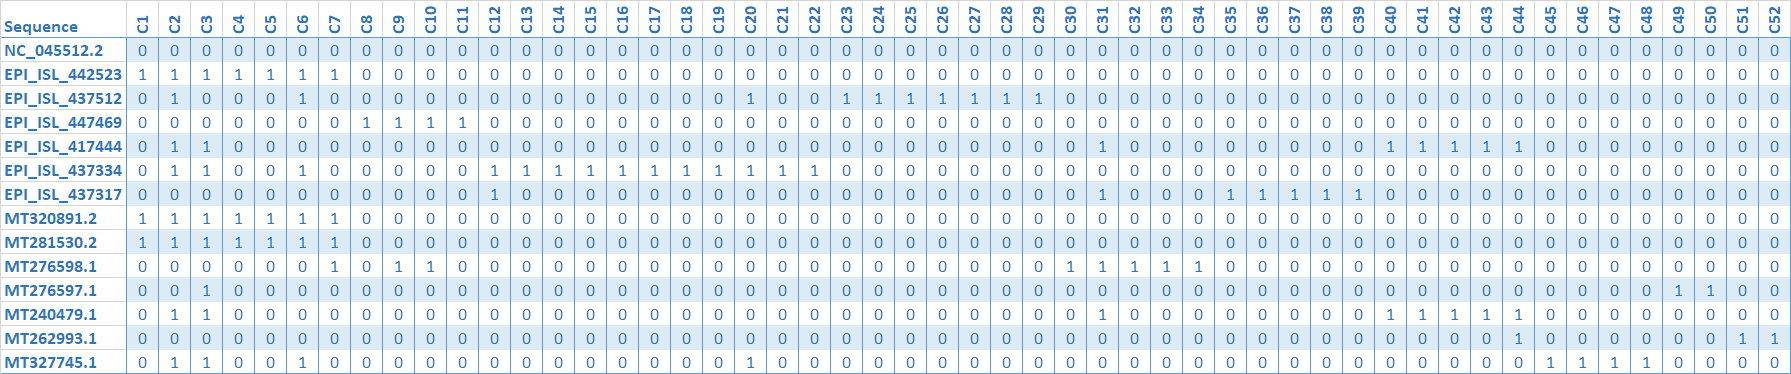
\includegraphics[width=1.6\linewidth]{character_table.png}}
  \caption{Albero di output del nostro script}
  \label{fig:script-tree}
\end{figure}
\noindent
Tuttavia per una filogenesi perfetta è necessario che la matrice utilizzata non sia una \lstinline{"matrice proibita"}, cioè che sia... % TODO: compleare.

La matrice in \cref{fig:matrix-perfect-phylo} è ottenuta applicando l'algoritmo descritto nel listato \ref{code:get_perfect_phylogeny_function} alla matrice di caratteri costruita in precedenza. Durante il procedimento vengono eliminate solamente 5 colonne, corrispondenti a cinque variazioni distinte.
\begin{figure}[H]
  \makebox[\textwidth][c]{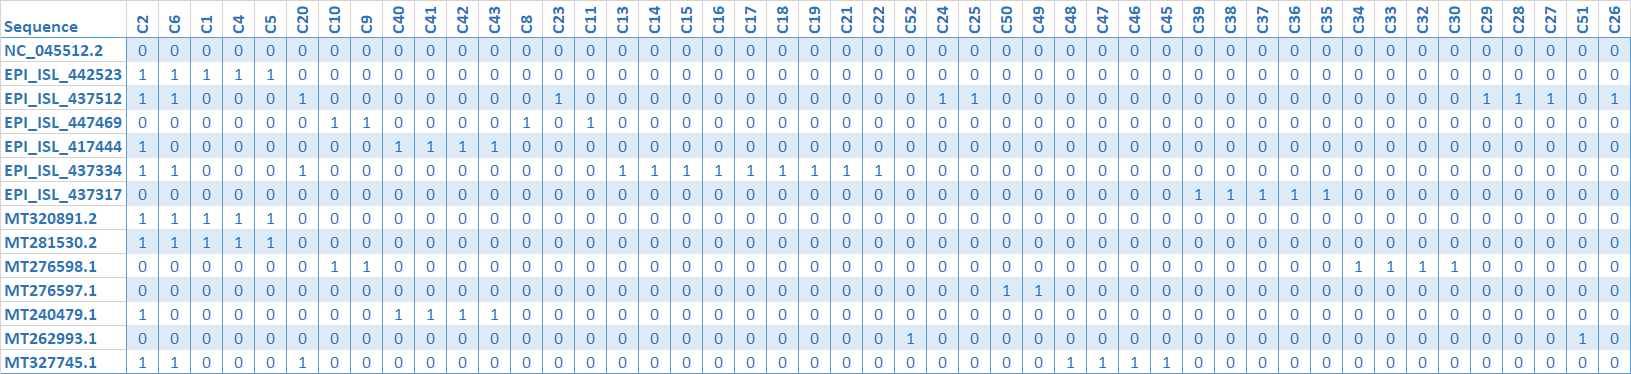
\includegraphics[width=1.6\linewidth]{perfect_phylogeny_table.png}}
  \caption{Matrice di caratteri per filogenesi perfetta}
  \label{fig:matrix-perfect-phylo}
\end{figure}

\newpage
\section{Algoritmo}
\subsection{Matrice delle variazioni}
Inizialmente, vengono recuperati gli identificativi delle 14 sequenze usate e caricati i file delle variazioni degli allineamenti generati in output nella prima parte del progetto:

\begin{lstlisting}[language=Python,caption=Caricamento dei file necessari per l'elaborazione,label=code:read_input_files]
reference_id = load_fasta_id(
  os.path.join('..', '..', 'project-1', 'input', 'reference.fasta')
)
sequence_ids = read_sequence_ids(paths=[
  os.path.join('..', '..', 'project-1', 'input', 'GISAID'),
  os.path.join('..', '..', 'project-1', 'input', 'ncbi'),
])
sequence_ids.insert(0, reference_id) #insert reference no variations

clustal_output = load_output('Clustal-NC_045512.2.json')
variations = clustal_output['unmatches'].items()
\end{lstlisting}

\noindent
L'algoritmo a partire dai file di output della prima parte del progetto genera una matrice binaria utilizzando come indici di riga gli identificativi delle sequenze e come colonne un identificativo univoco assegnato ad ogni variazione.

La matrice binaria così impostata contiene il valore \lstinline{1} qualora la variazione identificata dalla colonna sia presente nella sequenza identificata dalla riga, altrimenti il valore della cella sarà pari a \lstinline{0}.
Questa è salvata nel file \lstinline{character_table.csv}.

\begin{lstlisting}[caption=Generazione della matrice binaria di caratteri,label=code:creation table.csv,language=Python]
for key, value in variations:
  row = np.zeros(len(sequence_ids))
  indexes.append('C{}'.format(counter))
  for sequence in value['sequences']:
    row[sequence_ids.index(sequence)] = 1
  rows.append(row)
  counter += 1

trait_matrix = pd.DataFrame(rows, index=indexes, columns=sequence_ids, dtype=np.uint8).transpose()
trait_matrix = phylogeny.reorder_columns(trait_matrix, axis=0)
trait_matrix.to_csv(os.path.join('..', 'output', 'character_table.csv'))
\end{lstlisting}

\subsection{Filogenesi perfetta}
Prima di procedere con la creazione dell'albero è necessario verificare che la matrice binaria generata in precedenza sia valida per una filogenesi perfetta.

Il metodo riportato nel listato \ref{code:get_perfect_phylogeny_function} riporta il codice utilizzato
per costruire la matrice binaria più grande che non sia \lstinline{"matrice proibita"}.

\begin{lstlisting}[caption=Funzione di generazione della matrice binaria per filogenesi perfetta,label=code:get_perfect_phylogeny_function,language=Python]
def get_perfect_phylogeny_character_matrix(df):
  columns = df.columns
  candidate_matrix = df[columns[0:1]]
  for i in range(1, len(columns)):
    candidate_matrix = candidate_matrix.join(df[columns[i:i+1]])

    if phylogeny.is_forbidden_matrix(candidate_matrix):
      candidate_matrix = candidate_matrix.drop(labels=candidate_matrix.columns[-1], axis=1)

  return candidate_matrix
\end{lstlisting}

\subsection{Generazione dell'albero}
A questo punto è possibile procedere con la ricostruzione dell'albero filogenetico a partire dalla \lstinline{candidate_matrix} e utilizzando funzioni definite nel file \lstinline{phylogeny.py} per costruire e visualizzare in output l'albero della filogenesi.

\begin{lstlisting}[caption=Chiamata alla generazione dell'albero,label=code:tree_creation,language=Python]
candidate_matrix = get_perfect_phylogeny_character_matrix(trait_matrix)
phylogeny.build_tree(candidate_matrix)
\end{lstlisting}

\subsubsection{Creazione dell'albero}
\noindent
La generazione dell'albero viene svolta come segue:
\begin{enumerate}
  \item Ordinamento decrescente delle colonne del dataframe in base al numero di valori \lstinline{1} presenti.
\end{enumerate}
\begin{lstlisting}[caption=Ordinamento decrescente delle colonne,label=code:desc_column_sorting,language=Python]
sorted_axis = df.sum(axis=0).sort_values(ascending=False)
return df[sorted_axis.index]
\end{lstlisting}

\begin{enumerate}
  \setcounter{enumi}{1}
  \item A partire dal nodo \lstinline{root}, per ogni sequenza genera una sequenza di nodi uno per ogni variazione presente, collegandola alla variazione precedente o al nodo \lstinline{root}.

  Durante l'elaborazione delle sequenze successive, se esiste già un figlio del \lstinline{current_node} rappresentante la variazione attuale, questo viene riutilizzato, altrimenti viene creato un nuovo nodo e collegato come figlio di \lstinline{current_node}.
\end{enumerate}
\begin{lstlisting}[caption=Funzione di creazione dell'albero,label=code:tree_creation_function,language=Python]
root = Node('root', edges={})
for i, row in df.iterrows():
  current_node = root

  for j in range(len(row)):
    # If alteration is present in the current sequence
    if row.iloc[j]:
      # If current_node has a link to the variation with label=j
      if j in current_node.edges:
        # Follow the same path without creating new nodes
        current_node = current_node.edges[j]
      else:
        u = Node('U-{}'.format(row.index[j]), edges={})
        current_node.parent = current_node
        current_node.edges[j] = u
        current_node = u

  Node(i, parent=current_node)
\end{lstlisting}

\begin{enumerate}
  \setcounter{enumi}{2}
  \item Conversione dell'albero precedentemente generato in un \lstinline{newick_tree} elaborabile dalla libreria \lstinline{biopython.Phylo} usata per la visualizzazione.
\end{enumerate}

\begin{lstlisting}[caption=Funzione di conversione in Newick Tree,label=code:newick_tree_function,language=Python]
def to_newick_tree(node):
  if node.is_leaf:
    return node.name

  return '({})'.format(','.join([ to_newick_tree(child) for child in node.children ]))

newick_string = to_newick_tree(root)
tree = Phylo.read(io.StringIO(newick_string), 'newick')
\end{lstlisting}

\begin{enumerate}
  \setcounter{enumi}{3}
  \item Inserimento delle informazioni aggiuntive sulle sequenze nelle foglie dell'albero. Questo step non può essere effettuato durante la conversione a \lstinline{newick_tree} perché alcuni caratteri usati verrebbero interpretati come parte della struttura dell'albero, alterando il risultato finale.
\end{enumerate}
\begin{lstlisting}[caption=Funzione per l'inserimento dei dati nelle foglie dell'albero,label=code:merge_sequence_data_function,language=Python]
def merge_sequences_data(node, sequences_data):
  if node.is_terminal():
    data = sequences_data[node.name]
    node.name = '{}\n {} in {}'.format(node.name, data['date'], data['location'])
    return

  [ merge_sequences_data(child, sequences_data) for child in node.clades ]

root = newick_tree.clade
merge_sequences_data(root, sequences_data)
\end{lstlisting}

\begin{enumerate}
  \setcounter{enumi}{4}
  \item Salvataggio e visualizzazione dell'albero filogenetico finale.
\end{enumerate}
\begin{lstlisting}[caption=Salvataggio e visualizzazione dell'albero filogenetico finale,label=code:build_tree_function,language=Python]
fig = plt.figure(figsize=(10, 8))
ax = fig.add_subplot(1, 1, 1)

Phylo.draw(tree, do_show=False, axes=ax)

ax.set_xlabel('Number of alterations')
ax.set_ylabel('Sequences')
plt.tight_layout()
plt.savefig(os.path.join('..', 'output', 'phylogenetic-tree.png'))
plt.show()
\end{lstlisting}

\newpage
\section{Conclusioni}
L'albero generato con ClustalW in \cref{fig:tool-tree}, rispetto all'albero da noi prodotto (\cref{fig:script-tree}), riesce a ottenere un livello di dettaglio maggiore arrivando a scindere i rami terminanti con tre foglie da noi identificati.

Il nodo israeliano etichettato con \lstinline{MT276597.1} in entrambi gli alberi risulta distante dalle altre due sequenze israeliane. Questo potrebbe far presupporre che derivi da un ceppo diverso del virus o da un'area geografica differente.

Il nodo \lstinline{MT262993.1} presenta alterazioni differenti rispetto alle altre sequenze rilevate in Pakistan. Come già descritto in precedenza nella seconda parte del progetto, alcune di queste alterazioni risultano essere cancellazioni di porzioni di basi per noi riconducibili ad un errore in fase di sequenziamento.

I rami restanti dell'albero in \cref{fig:script-tree} mostrano come nella stessa area geografica i genomi siano simili tra loro il che ci porta a ipotizzare che la diffusione all'interno del paese si sia sviluppata a partire da un singolo paziente per nazione e non da pazienti contagiati da mutazioni diverse del virus.

Analizzando l'albero, i ceppi \textit{iraniani} e \textit{turchi} presentano mutazioni comuni. Inoltre, le sequenze di entrambi i paesi condividono una variazione con il ceppo \textit{pakistano}.
Il ceppo di virus rilevato in \textit{Israele} sembra avere un'origine differente e non condivide mutazioni simili con le sequenze degli altri paesi analizzati.

\vspace{2mm}
\noindent
In conclusione, gli alberi ottenuti in \cref{fig:script-tree,fig:tool-tree} risultano abbastanza simili, tuttavia presentano alcune differenze.

Ipotizziamo che queste derivino principalmente dal fatto che l'albero in \cref{fig:script-tree} è costruito basandosi sul numero di alterazioni rispetto alla sequenza reference.
Al contrario, l'albero in \cref{fig:tool-tree} è generato in base alla distanza tra le \textit{intere} sequenze a partire da un allineamento.

\newpage
\begin{figure}[H]
  \makebox[\textwidth][c]{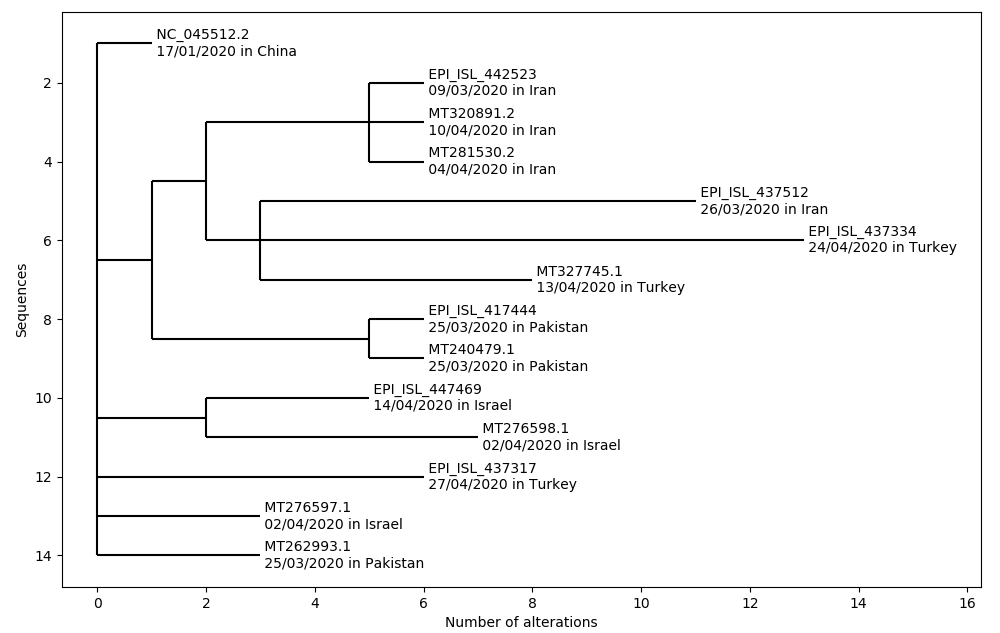
\includegraphics[width=1.1\linewidth]{perfect-phylogeny.png}}
  \caption{Albero di output del nostro script}
  \label{fig:script-tree}
\end{figure}
\begin{figure}[H]
  \makebox[\textwidth][c]{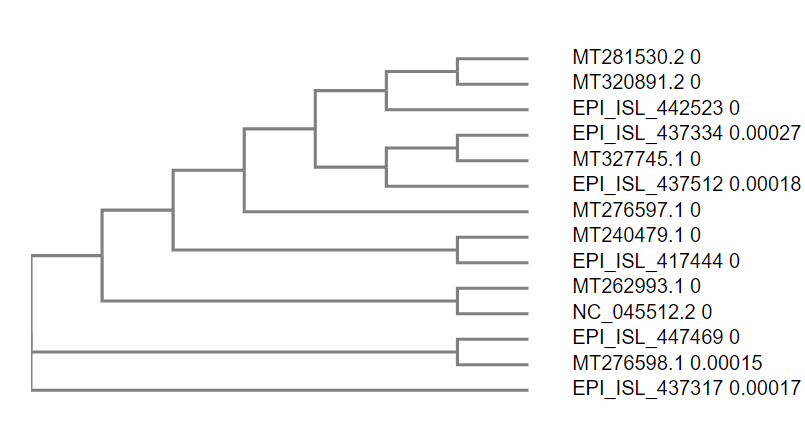
\includegraphics[width=1\linewidth]{ncbi_tree.png}}
  \caption{Albero di output derivato dall'allineamento con ClustalW}
  \label{fig:tool-tree}
\end{figure}

\newpage
\section{Divisone del lavoro}
Durante la realizzazione del progetto entrambi i componenti del gruppo hanno partecipato attivamente alla sua realizzazione. In particolare:
\begin{itemize}
  \item \textbf{Edoardo Silva} si è occupato principalmente di recuperare i file esterni da elaborare e confrontare.
  \item \textbf{Davide Marchetti} si è occupato principalmente di generare i file di output.
  \item Entrambi hanno lavorato alla creazione ed elaborazione della matrice e dell'albero, con tutte le funzioni ausiliarie allo scopo del progetto.
\end{itemize}

\end{document}